\documentclass[10pt,a4paper]{article}
\usepackage[utf8]{inputenc}
\usepackage{amsmath}
\usepackage{amsfonts}
\usepackage{amssymb}
\usepackage{graphicx}
\usepackage{epstopdf}
\usepackage[ngerman]{babel}
\usepackage[ngerman]{translator}
\usepackage[colorlinks=true,
        linkcolor=black,
        citecolor=black,
        filecolor=black,
        pagecolor=black,
        urlcolor=black,
        bookmarks=true,
        bookmarksopen=true,
        bookmarksopenlevel=3,
        plainpages=false,
        pdfpagelabels=true]{hyperref}

%Paket laden
\usepackage[
	nonumberlist, %keine Seitenzahlen anzeigen
	acronym,      %ein Abkürzungsverzeichnis erstellen
	toc,          %Einträge im Inhaltsverzeichnis
	section]      %im Inhaltsverzeichnis auf section-Ebene erscheinen
	{glossaries}

%Befehle für Glossar
\makeglossaries
\newglossaryentry{Feld}{
	name=Feld,
	description={Ein Feld ist eine quadratische Fläche mit einem Steitenmaß von mindestens 10cm. Es stellt die kleinste Einheit eines
	Spielfeldes dar}
}

\parindent 0pt
\pagestyle{headings}

\let\oldsection\section
\renewcommand{\section}{\newpage \oldsection}

\title{
	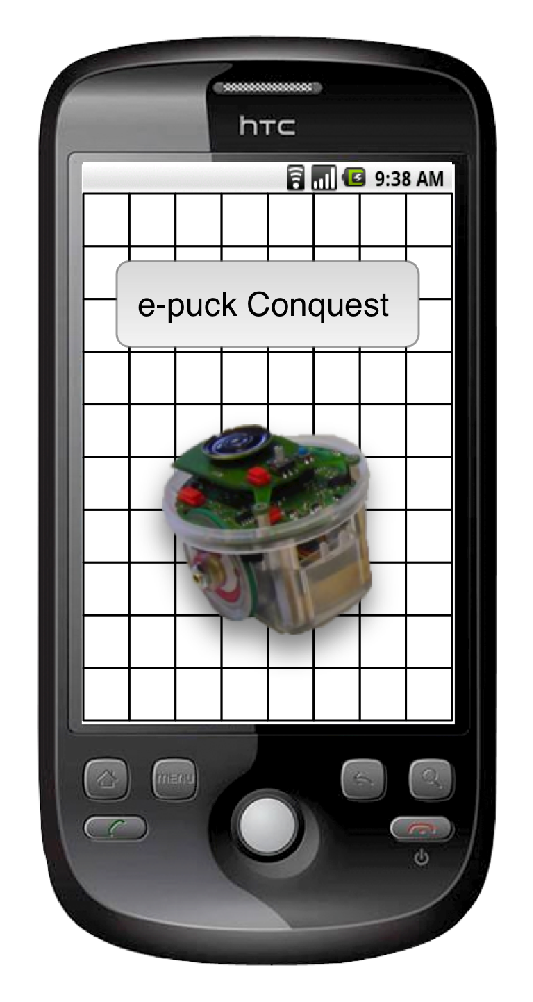
\includegraphics[height=10cm]{logo.eps} \\
	\vspace{1cm}
	Entwurf
}
\author{SEP - ITS - Team \\ Max Binder, Florian Bürchner, Martin Freund, \\Florian Lorenz,
											Andreas Poxrucker, Andreas Wilhelm}
\begin{document}
	\maketitle
	\newpage
	\tableofcontents	
	\newpage

	\section{Einleitung}
		Dieses Dokument stellt den konzeptionellen Entwurf des e-puck Conquest Systems dar. Hierbei handelt es sich um ein
		verteiltes System mit bis zu sechs  e-puck Roboter und einem Android-Smartphone. \\
		Die Roboter haben die Aufgabe ein Spielfeld möglichst zeiteffizient in Kooperation mit den anderen Teilnehmern zu erkunden.
		Auf dem Smartphone werden die gesammelten Kartendaten dargestellt, außerdem kann ein e-puck zur manuellen Steuerung
		ausgewählt werden. \\
		Die Kommunikation der Roboter wird über ein Bluetooth-Netzwerk in Ringarchitektur behandelt (siehe Abbildung 1). Trotz
		der Beschränkung des Bluetooth-Moduls auf 7 direkte Verbindungen wird durch diese Architektur eine hohe Skalierbarkeit
		gewährleistet. Das Smartphone verbindet sich zu einem ausgewählten e-puck, Nachrichten werden über Broadcast über
		das Netzwerk an alle anderen Teilnehmer versendet.
		\begin{figure}[h]
			\centering
			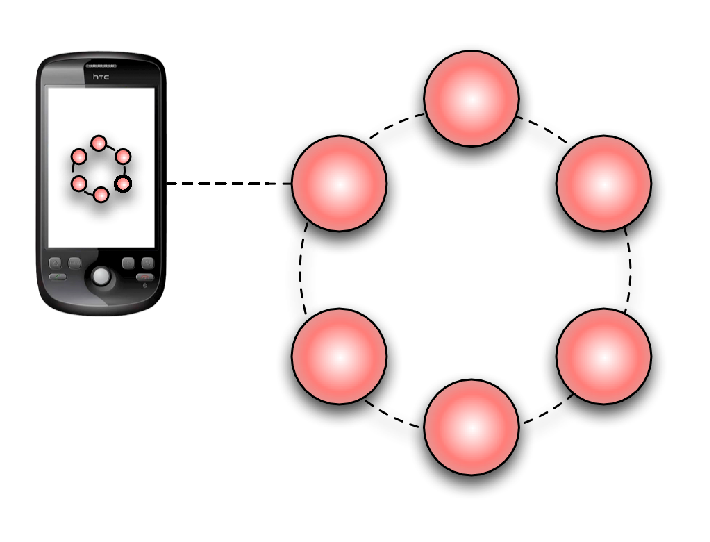
\includegraphics[width=10cm]{images/system.eps}
  			\caption{Verteiltes e-puck System}
  		\end{figure} \\
		Der Entwurf des Systems wird zur besseren Übersicht in die Bereiche \textit{e-puck Roboter}, \textit{Smartphone} und
		\textit{Kommunikation} aufgeteilt. Das Ziel ist ein möglichst hohes Maß an	Qualität, Wartbarkeit und Erweiterbarkeit. Dazu ist
		ein sinnvolles Systemdesign unter Verwendung mehrerer Entwurfsmuster und Architekturen in allen Bereichen erforderlich. \\
		Weiterhin werden in den folgenden Abschnitten Datentypen und Schnittstellen der Komponenten erläutert. Die beschränkten
		Ressourcen der Roboter erzwingen hierbei einen möglichst effizienten Aufbau. Insbesondere stellt der interne
		Arbeitsspeicher sowie die Rechenleistung der e-pucks eine Einschränkung für den Entwurf dar.
				
	\section{e-Puck Roboter}	
	
		\subsection{Architektur}
		Die Software des e-puck wird als Schichtenarchitektur mit wachsendem Abstraktionsgrad entworfen. \\
		Jede Schicht besteht aus einer oder mehreren Komponenten. Teilweise sind diese Komponenten wiederum aus mehreren
		Schichten. \\
		
		Die folgenden Abschnitte beschreiben die einzelnen Komponenten des Diagramms näher.
		 
			\subsection{Komponente `Interrupt'}
			Die Komponente Interrupt 
			\subsection{Komponente `Timer'}
			
			\subsection{Komponente `Communication'}
			
			\subsection{Komponente `Motor'}
			
			\subsection{Komponente `ADC'}
			
			\subsection{Komponente `I2C'}
			
			\subsection{Komponente `IR proximity sensor'}
			
			\subsection{Komponente `Line sensor'}
			
			\subsection{Komponente `Selector'}
			
			\begin{figure}[h]
			\centering
			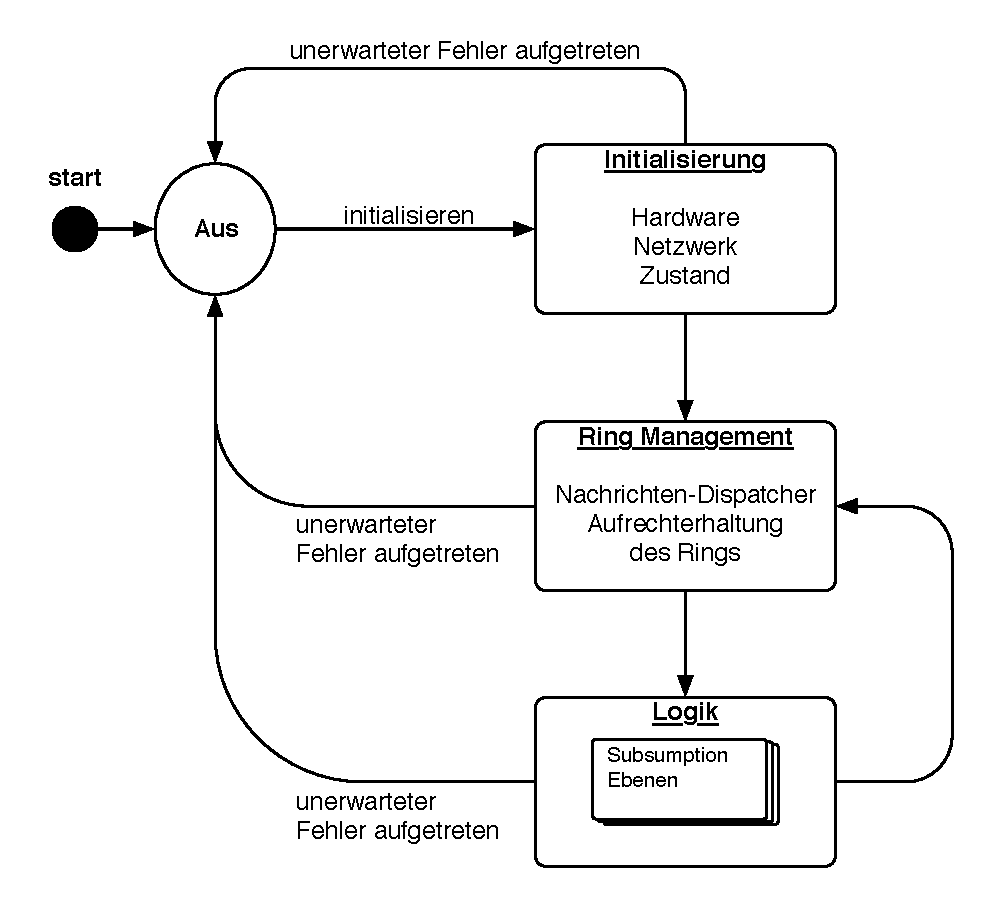
\includegraphics[width=10cm]{images/e-puck.eps}
  			\caption{Ablaufdiagramm}
  		\end{figure}	
	\section{Smartphone}
	\section{Kommunikation}
				
	\newpage	
	%Glossar ausgeben
	\printglossary[style=altlist,title=Glossar]
						
\end{document}